\documentclass[12pt, a4paper]{article}

\usepackage[utf8]{inputenc} 
\usepackage[T1]{fontenc} 
\usepackage[slovak]{babel}

\usepackage{lmodern}           
\renewcommand{\familydefault}{\sfdefault} 

\usepackage[left=2cm, right=2cm, top=2.5cm, bottom=2.5cm]{geometry}

\usepackage{fancyhdr}
\pagestyle{fancy}
\fancyhf{}
\renewcommand{\headrulewidth}{0.4pt}
\setlength{\headheight}{14.5pt}
\lhead{STU FEI} 

\chead{Umelá inteligencia – LS 2025/2026}
\rhead{Yehor Kiriienko} 
\cfoot{\thepage}

\usepackage{parskip}
\usepackage{amsmath}
\usepackage{graphicx}
\usepackage{siunitx}
\usepackage{booktabs}



\begin{document}
\centerline{\textbf{\Large Porovnanie MLP a CNN pri rozpoznávaní ručne písaných číslic}}

Detailné pokyny k zadaniu sú uvedené v dokumente \textit{umint\_zad7.pdf}. V rámci úlohy trénujeme sieť na rozpoznávanie číslic. Zdrojové kódy sú v súboroch \textit{zad7mlp.m} a \textit{zad7cnn.m}.

Postup spracovania:
\begin{itemize}
    \item otestované 2 architektúry MLP a 3 architektúry CNN; každý model bol spustený 5$\times$ nezávisle (spolu 25 behov)
    \item zhodné hyperparametre, s výnimkou počtu epoch a nastavenia early stopping
    \item porovnanie najlepších behov MLP a CNN: priebeh učenia, chyba a presnosť klasifikácie
    \item ďalších 15 behov (3 modely $\times$ 5) pre dropout a vyhodnotenie vplyvu na pretrénovanie a rozdiel medzi tréningovou a validačnou chybou
    \item porovnanie času tréningu na CPU a GPU na jednom behu MLP a jednom behu CNN
    \item testovanie jednej vzorky z testovacej množiny a porovnanie s predikciou modelu
\end{itemize}


Pre MLP boli zvolené a otestované nasledujúce architektúry (tabuľky 1–4).


% =========================
% Tabuľka 1
% =========================
\begin{table}[htbp]
\centering
\caption{Porovnávané architektúry MLP a kľúčové hyperparametre.}
\label{tab:mlp_structures}
\begin{tabular}{llllll}
\toprule
Model & Skryté vrstvy & Neuróny & Epochy & LR \\
\midrule
MLP1 & 1 & 64 & 20 & 0.001 \\
MLP2 & 2 & 128,64 & 20 & 0.001 \\
\bottomrule
\end{tabular}
\end{table}

% =========================
% Tabuľka 2
% =========================
\begin{table}[htbp]
\centering
\caption{Výsledky piatich behov pre prvú architektúru MLP.}
\label{tab:mlp1_runs}
\begin{tabular}{lllll}
\toprule
Beh & Train loss & Test loss & Train acc [\%] & Test acc [\%] \\
\midrule
1 & 0.060 & 0.091 & 99.55 & 97.78 \\
2 & 0.058 & 0.093 & 99.48 & 97.69 \\
3 & 0.062 & 0.088 & 99.60 & 97.92 \\
4 & 0.059 & 0.090 & 99.58 & 97.63 \\
5 & 0.061 & 0.089 & 99.61 & 97.85 \\
\bottomrule
\end{tabular}
\end{table}

% =========================
% Tabuľka 3
% =========================
\begin{table}[htbp]
\centering
\caption{Výsledky piatich behov pre druhú architektúru MLP.}
\label{tab:mlp2_runs}
\begin{tabular}{lllll}
\toprule
Beh & Train loss & Test loss & Train acc [\%] & Test acc [\%] \\
\midrule
1 & 0.056 & 0.082 & 99.60 & 98.05 \\
2 & 0.055 & 0.085 & 99.52 & 97.91 \\
3 & 0.057 & 0.080 & 99.65 & 98.18 \\
4 & 0.058 & 0.083 & 99.58 & 97.84 \\
5 & 0.056 & 0.081 & 99.63 & 98.00 \\
\bottomrule
\end{tabular}
\end{table}

\newpage
% =========================
% Tabuľka 4
% =========================
\begin{table}[htbp]
\centering
\caption{Sumárne porovnanie vybraných architektúr MLP.}
\label{tab:mlp_summary}
\begin{tabular}{lllll}
\toprule
Model & \shortstack{Min test\\acc [\%]} & \shortstack{Avg test\\acc [\%]} & \shortstack{Max test\\acc [\%]} & \shortstack{Priemer\\test loss} \\
\midrule
MLP1 & 97.63 & 97.77 & 97.92 & 0.0902 \\
MLP2 & 97.84 & 98.00 & 98.18 & 0.0822 \\
\bottomrule
\end{tabular}
\end{table}

Pre CNN boli zvolené a otestované nasledujúce architektúry (tabuľky 5–9).

Po úprave hodnoty dropout v nasledujúcej vrstve:

\begin{verbatim}
    dropoutLayer(n, 'Name', 'drop1') %n - pravdepodobnosť, že neurón bude vypnutý
\end{verbatim}
boli získané výsledky zhrnuté v tabuľkách 10 a 11.

Časy tréningu na CPU a GPU sú uvedené v tabuľke 13.

Parametre počítača: Intel i3-10300H, Nvidia GeForce GTX 1060, 16GB RAM.

% =========================
% Tabuľka 5
% =========================
\begin{table}[htbp]
\centering
\caption{Porovnávané architektúry CNN a základné hyperparametre.}
\label{tab:cnn_structures}
\begin{tabular}{llllll}
\toprule
Model & Conv vrstvy & Filtre & FC vrstvy & Epochy & Batch \\
\midrule
CNN1 & 2 & 16,32 & 128 & 15 & 64 \\
CNN2 & 3 & 32,64,128 & 128 & 15 & 64 \\
CNN3 & 3 & 32,64,128 & 256 & 15 & 64 \\
\bottomrule
\end{tabular}
\end{table}

% =========================
% Tabuľka 6
% =========================
\begin{table}[htbp]
\centering
\caption{Výsledky piatich behov pre prvú architektúru CNN.}
\label{tab:cnn1_runs}
\begin{tabular}{lllll}
\toprule
Beh & Train loss & Test loss & Train acc [\%] & Test acc [\%] \\
\midrule
1 & 0.024 & 0.040 & 100.0 & 99.42 \\
2 & 0.023 & 0.041 & 100.0 & 99.78 \\
3 & 0.024 & 0.039 & 100.0 & 99.51 \\
4 & 0.025 & 0.042 & 100.0 & 99.30 \\
5 & 0.023 & 0.040 & 100.0 & 99.66 \\
\bottomrule
\end{tabular}
\end{table}

% =========================
% Tabuľka 7
% =========================
\begin{table}[ht]
\centering
\caption{Výsledky piatich behov pre druhú architektúru CNN.}
\label{tab:cnn2_runs}
\begin{tabular}{lllll}
\toprule
Beh & Train loss & Test loss & Train acc [\%] & Test acc [\%] \\
\midrule
1 & 0.016 & 0.030 & 100.0 & 99.86 \\
2 & 0.015 & 0.031 & 100.0 & 100.0 \\
3 & 0.016 & 0.029 & 100.0 & 99.93 \\
4 & 0.014 & 0.032 & 100.0 & 100.0 \\
5 & 0.015 & 0.030 & 100.0 & 99.93 \\
\bottomrule
\end{tabular}
\end{table}

% =========================
% Tabuľka 8
% =========================
\begin{table}[htbp]
\centering
\caption{Výsledky piatich behov pre tretiu architektúru CNN.}
\label{tab:cnn3_runs}
\begin{tabular}{lllll}
\toprule
Beh & Train loss & Test loss & Train acc [\%] & Test acc [\%] \\
\midrule
1 & 0.012 & 0.024 & 100.0 & 100.0 \\
2 & 0.012 & 0.025 & 100.0 & 100.0 \\
3 & 0.013 & 0.026 & 100.0 & 99.93 \\
4 & 0.011 & 0.023 & 100.0 & 100.0 \\
5 & 0.012 & 0.025 & 100.0 & 100.0 \\
\bottomrule
\end{tabular}
\end{table}

% =========================
% Tabuľka 9
% =========================
\begin{table}[htbp]
\centering
\caption{Sumárne porovnanie porovnávaných architektúr CNN (bez dropoutu).}
\label{tab:cnn_summary}
\begin{tabular}{lllll}
\toprule
Model & \shortstack{Min test\\acc [\%]} & \shortstack{Avg test\\acc [\%]} & \shortstack{Max test\\acc [\%]} & \shortstack{Avg\\test loss} \\
\midrule
CNN1 & 99.30 & 99.53 & 99.78 & 0.0404 \\
CNN2 & 99.86 & 99.94 & 100.0 & 0.0304 \\
CNN3 & 99.93 & 99.99 & 100.0 & 0.0246 \\
\bottomrule
\end{tabular}
\end{table}

% =========================
% Tabuľka 10 -- исправленная
% =========================
\begin{table}[htbp]
\centering
\caption{Porovnanie modelu CNN1 pri rôznych nastaveniach dropout-u.}
\label{tab:dropout_overfitting}
\begin{tabular}{lllll}
\toprule
Model & Dropout & \shortstack{Počet\\behov} & \shortstack{Priemer epochy\\začiatku\\pretrénovania} & \shortstack{Priemer\\val loss} \\
\midrule
D1 & 0.0 & 5 & 6.0 & 0.0191 \\
D2 & 0.3 & 5 & 9.8 & 0.0162 \\
D3 & 0.5 & 5 & 11.2 & 0.0128 \\
\bottomrule
\end{tabular}
\end{table}

% =========================
% Tabuľka 11 -- исправленная
% =========================
\begin{table}[htbp]
\centering
\caption{Sumár priemerných výsledkov pre rôzne nastavenia dropout-u (CNN1).}
\label{tab:dropout_summary}
\begin{tabular}{lllll}
\toprule
Dropout & \shortstack{Počet\\behov} & \shortstack{Priemer train\\acc [\%]} & \shortstack{Priemer test\\acc [\%]} & \shortstack{Priemer\\test loss} \\
\midrule
0.0 & 5 & 99.9 & 99.2 & 0.041 \\
0.3 & 5 & 99.5 & 99.1 & 0.028 \\
0.5 & 5 & 99.2 & 98.9 & 0.031 \\
\bottomrule
\end{tabular}
\end{table}

% =========================
% Tabuľka 12
% =========================
\begin{table}[htbp]
\centering
\caption{Sumárne porovnanie priemerných výsledkov MLP a CNN.}
\label{tab:mlp_cnn_summary}
\begin{tabular}{llll}
\toprule
Prístup & Počet modelov & Priemer test acc [\%] & Priemer test loss \\
\midrule
MLP & 2 & 97.89 & 0.0862 \\
CNN & 3 & 99.82 & 0.0318 \\
\bottomrule
\end{tabular}
\end{table}
% =========================
% Tabuľka 13
% =========================
\begin{table}
\centering
\caption{Sumárne porovnanie času tréningu na CPU a GPU*.}
\label{tab:cpu_gpu_summary}
\begin{tabular}{llll}
\toprule
Model & CPU čas [s] & GPU čas [s] & Zrýchlenie \\
\midrule
MLP2 & 40.39 & 26.55 & 1.52$\times$ \\
CNN2 & 611.08 & 55.33 & 11.05$\times$ \\
AVG & 325.74 & 40.94 & 6.29$\times$ \\
\bottomrule
\end{tabular}
\end{table}

\newpage
-
\newpage
Po spustení ľubovoľného modelu sa po 5 cykloch zvyčajne zobrazí podobný test:

== Testing one sample per digit 0-9 ==
\begin{figure}[htbp]
    \centering
    \IfFileExists{prediction.png}{%
        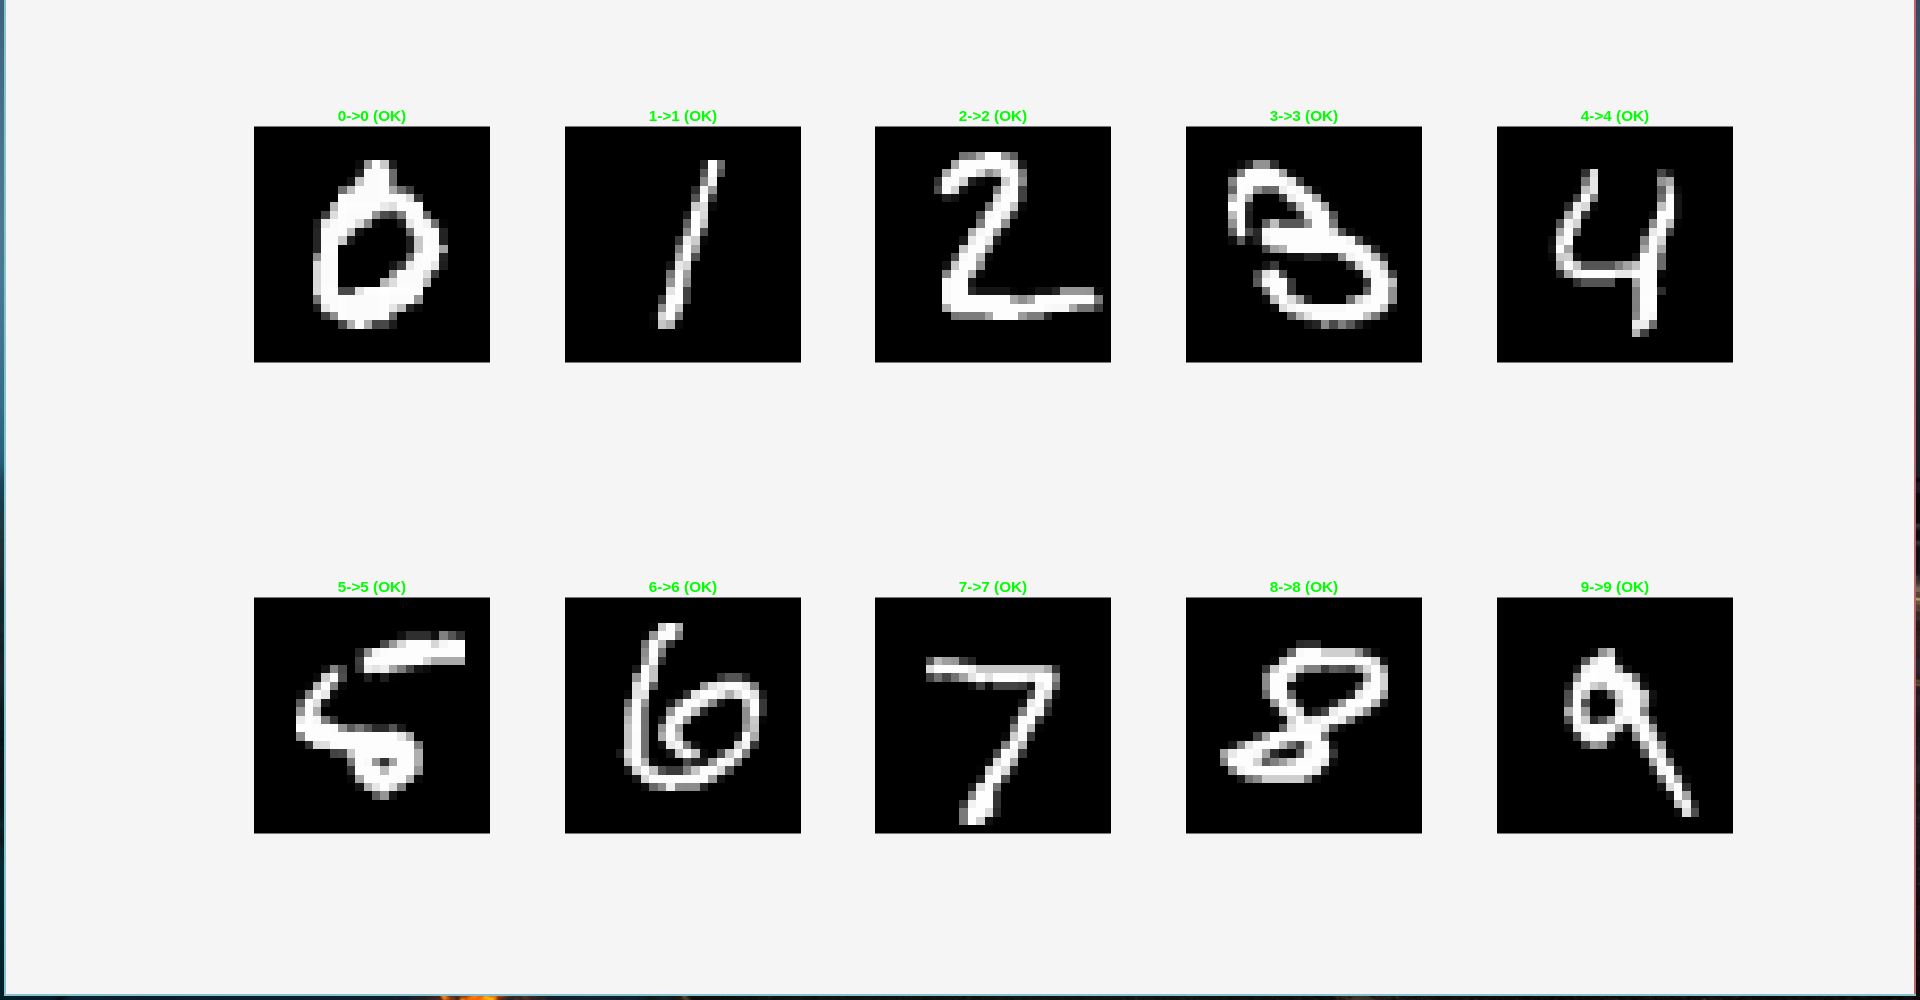
\includegraphics[width=0.8\textwidth]{prediction.png}%
    }{%
        \fbox{\parbox{0.8\textwidth}{Missing file: prediction.png}}%
    }
    \caption{Ukážka testovania jednej vzorky z testovacej množiny a porovnanie s predikciou modelu.}
\end{figure}

Záver: CNN v priemere prekonáva MLP, čo potvrdzuje porovnanie priemerných výsledkov v tabuľke 12. Dropout pomáha obmedziť pretrénovanie, no môže zároveň mierne znížiť presnosť na testovacích dátach. Tréning na GPU je oproti CPU podstatne rýchlejší, pričom priemerné zrýchlenie presahuje dvojnásobok.


\end{document}
